\begin{center}
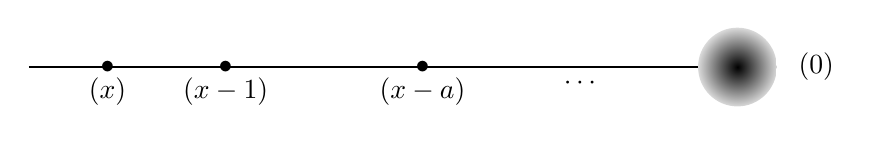
\begin{tikzpicture}

% Affine line
\draw[thick] (0,0)
    -- (1,0) node {$\bullet$} node[below] {$(x)$}
    -- (2.5,0) node {$\bullet$} node[below] {$(x-1)$}
    -- (5,0) node {$\bullet$} node[below] {$(x-a)$}
    -- (7,0) node[below] {$\cdots$}
    -- (9,0);


% Generic point
\shade[inner color=black, outer color=gray!30]
    (9,0) circle (0.5);
\draw (10,0) node {$(0)$};
\end{tikzpicture}
\end{center}